\documentclass{article}

\usepackage{graphicx}
\usepackage{tikz}
\usepackage{tikzsymbols}
\usetikzlibrary{calc,patterns,shapes.geometric}
\pagestyle{empty}
\usepackage[margin=0pt]{geometry}
\geometry{papersize={14in,12in}}

\def\centerarc[#1](#2)(#3:#4:#5){\draw[#1] ($(#2)+({#5*cos(#3)},{#5*sin(#3)})$) arc (#3:#4:#5);}

\begin{document}
	\begin{figure}
		\centering
		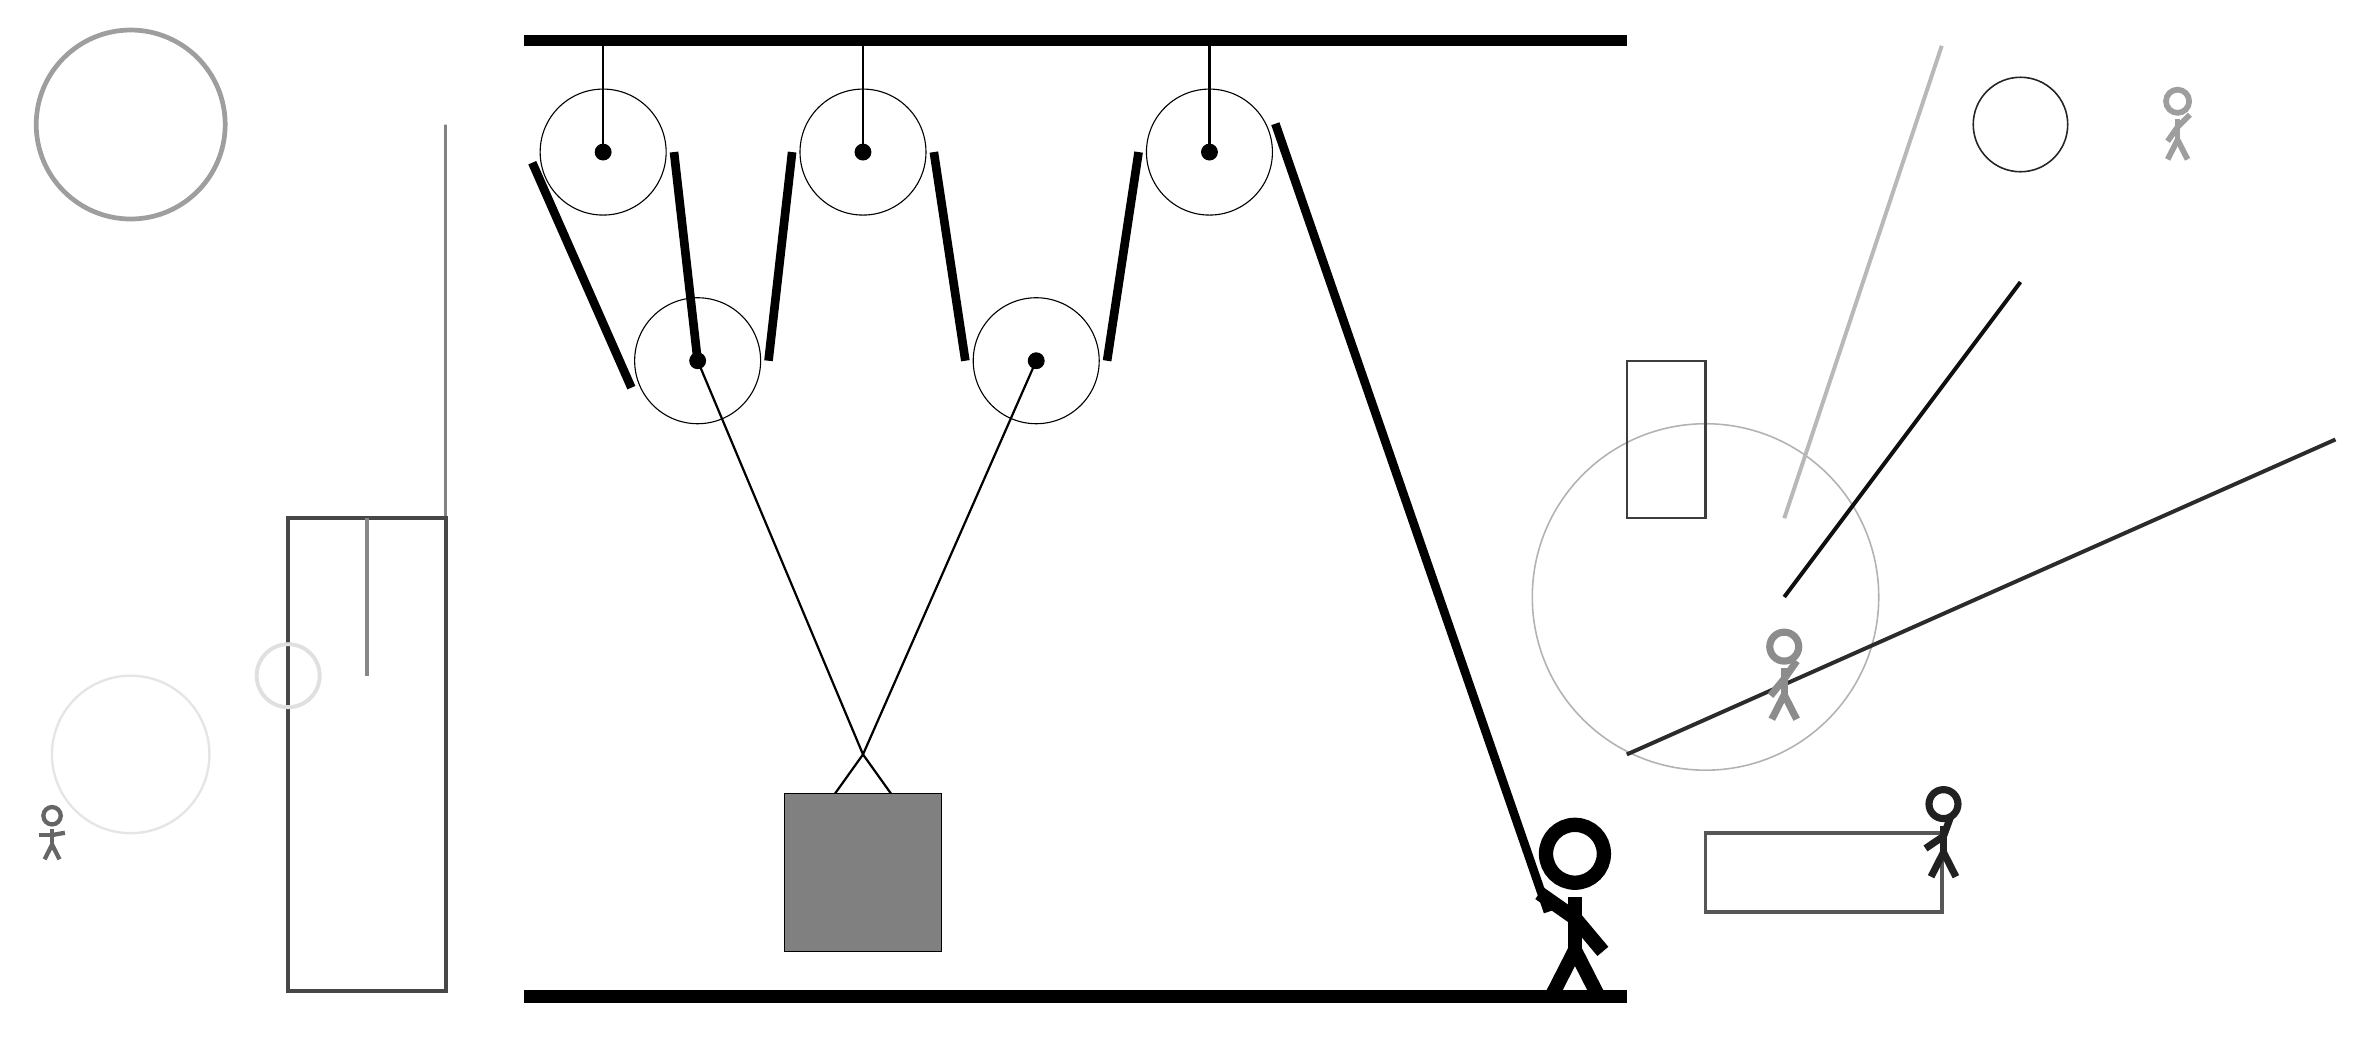
\begin{tikzpicture}
			%%%%% START %%%%%
			
			\draw[fill=black] (-2, 9) rectangle (12, 9.125);
			
			\draw (-1, 7.65) circle (0.8);
			\draw[fill=black] (-1, 7.65) circle (0.1);
			\draw[thick] (-1, 7.65) -- (-1, 9);
			
			\draw [line width=0.3mm, color=black!10](-7, 0) circle (1.0);
			
			\draw[line width=0.4mm, color=black!49] (-3, -1) rectangle (-3, 8);
			\draw[line width=0.5mm, color=black!72] (-3, -3) rectangle (-5, 3);
			\draw [line width=0.2mm, color=black!30](13, 2) circle (2.2);
			
			\draw[line width=0.5mm, color=black!66] (13, -2) rectangle (16, -1);
			\draw [line width=0.5mm, color=black!12](-5, 1) circle (0.4);
			\draw [line width=0.6mm, color=black!38](-7, 8) circle (1.2);
			
			\draw[line width=0.5mm, color=black!47](-4, 3) -- (-4, 1);
			\draw [line width=0.2mm, color=black!86](17, 8) circle (0.6);
			
			\node[line width=0.2mm, color=black!38] at (19, 8) {\Strichmaxerl[4][55][45]};
			
			\node[line width=0.7mm, color=black!87] at (16, -1) {\Strichmaxerl[5][34][70]};
			\draw[line width=0.5mm, color=black!28](16, 9) -- (14, 3);
			\draw[line width=0.5mm, color=black!94](14, 2) -- (17, 6);
			
			\draw[line width=0.3mm, color=black!76] (13, 3) rectangle (12, 5);
			\draw[line width=0.5mm, color=black!83](12, 0) -- (21, 4);
			\node[line width=0.2mm, color=black!45] at (14, 1) {\Strichmaxerl[5][51][55]};
			\node[line width=0.2mm, color=black!60] at (-8, -1) {\Strichmaxerl[3][0][10]};
			
			\draw (2.3, 7.65) circle (0.8);
			\draw[fill=black] (2.3, 7.65) circle (0.1);
			\draw[thick] (2.3, 7.65) -- (2.3, 9);
			
			\draw (6.7, 7.65) circle (0.8);
			\draw[fill=black] (6.7, 7.65) circle (0.1);
			\draw[thick] (6.7, 7.65) -- (6.7, 9);
			
			\draw (0.2, 5) circle (0.8);
			\draw[fill=black] (0.2, 5) circle (0.1);
			
			\draw (4.5, 5) circle (0.8);
			\draw[fill=black] (4.5, 5) circle (0.1);
			
			\draw[thick] (0.2, 5) -- (2.3, 0)  -- (4.5, 5);
			\draw[thick]  (1.8, -0.7) -- (2.3, 0) -- (2.8, -0.7);
			\draw[fill=black!50] (1.3, -0.5) rectangle (3.3, -2.5);
			
			\draw[line width=1.1mm] (0.2, 5) -- (-0.1, 7.65);
			\centerarc[line width=1.1mm](-1, 7.65)(0:200:0.9);
			\draw[line width=1.1mm] (-1.9, 7.515) -- (-0.6415, 4.658);
			\centerarc[line width=1.1mm](0.2, 5)(200:360:0.9);
			\draw[line width=1.1mm](1.1, 5) -- (1.4, 7.65);
			\centerarc[line width=1.1mm](2.3, 7.65)(0:180:0.9);
			\draw[line width=1.1mm] (3.2, 7.65) -- (3.6, 5);
			\centerarc[line width=1.1mm](4.5, 5)(180:360:0.9);
			\draw[line width=1.1mm] (5.4, 5) -- (5.8, 7.65);
			\centerarc[line width=1.1mm](6.7, 7.65)(20:180:0.9);
			\draw[line width=1.1mm](7.537, 8.01)  -- (11, -2);
			
			\node at (11.3, -2) {\Strichmaxerl[10][-35][-50]};
			
			\draw[fill=black] (-2, -3) rectangle (12, -3.15);
			
			%%%%% END %%%%%
		\end{tikzpicture}
	\end{figure}	
\end{document}